\section{Results: what does a crop loss mean for nutrient supply?}\label{sec:nutrition}

\subsection{What each crop supplies}
\begin{figure}[H]\centering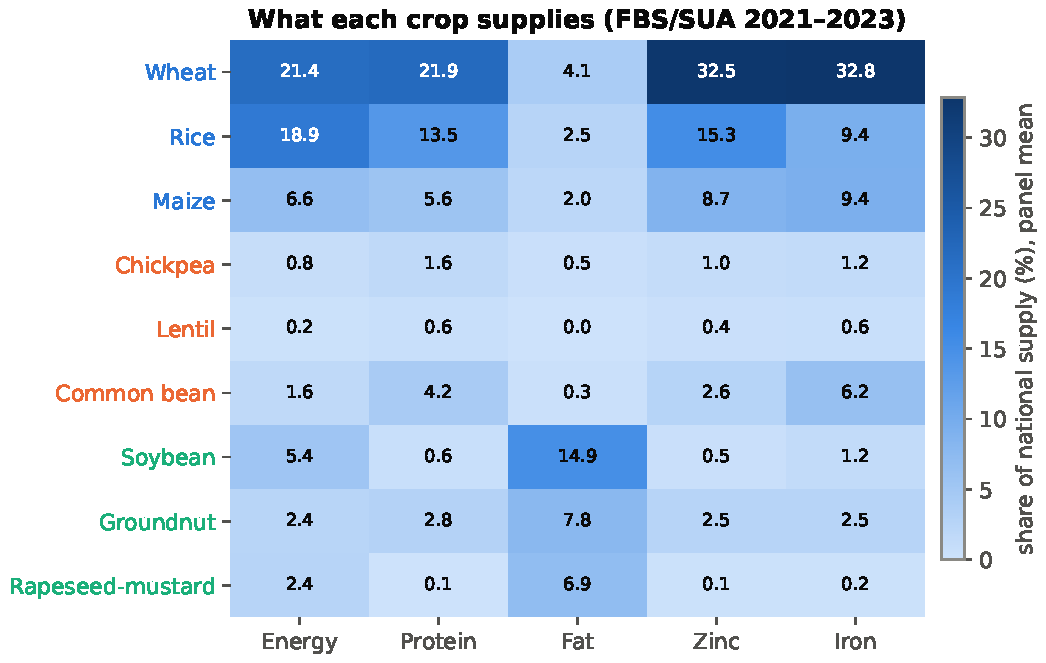
\includegraphics[width=0.8\linewidth]{G07_nutrient_profiles.pdf}
\caption{Share of national supply of each nutrient from each crop (mean over the crop's panel countries, FBS 2021--23).}\label{fig:profiles}\end{figure}
\begin{itemize}
\item \textbf{Cereals} dominate energy, protein, zinc and iron.
\item \textbf{Oilseeds} mainly supply fat, as oil. Soybean is mostly crushed, so the FBS credit it with almost no
food protein.
\item \textbf{Pulses} matter for protein and iron, mostly in South Asia and East Africa (Figure~\ref{fig:profiles}).
\end{itemize}

\subsection{Adequacy}
Iron is the nutrient most often below requirement: \nIronShort\ of \nAdqCountries\ panel countries under the main
requirement. Energy, protein, fat and zinc are below requirement in none (Table~\ref{tab:adequacy}). The iron
result depends on the requirement chosen: with iron at 15\% bioavailability, \nIronShortAlt\ countries fall short.
Section~\ref{sec:adequacy} explains why national ratios are a supply-side screen.

\subsection{A standard 10\% yield loss}
\begin{figure}[H]\centering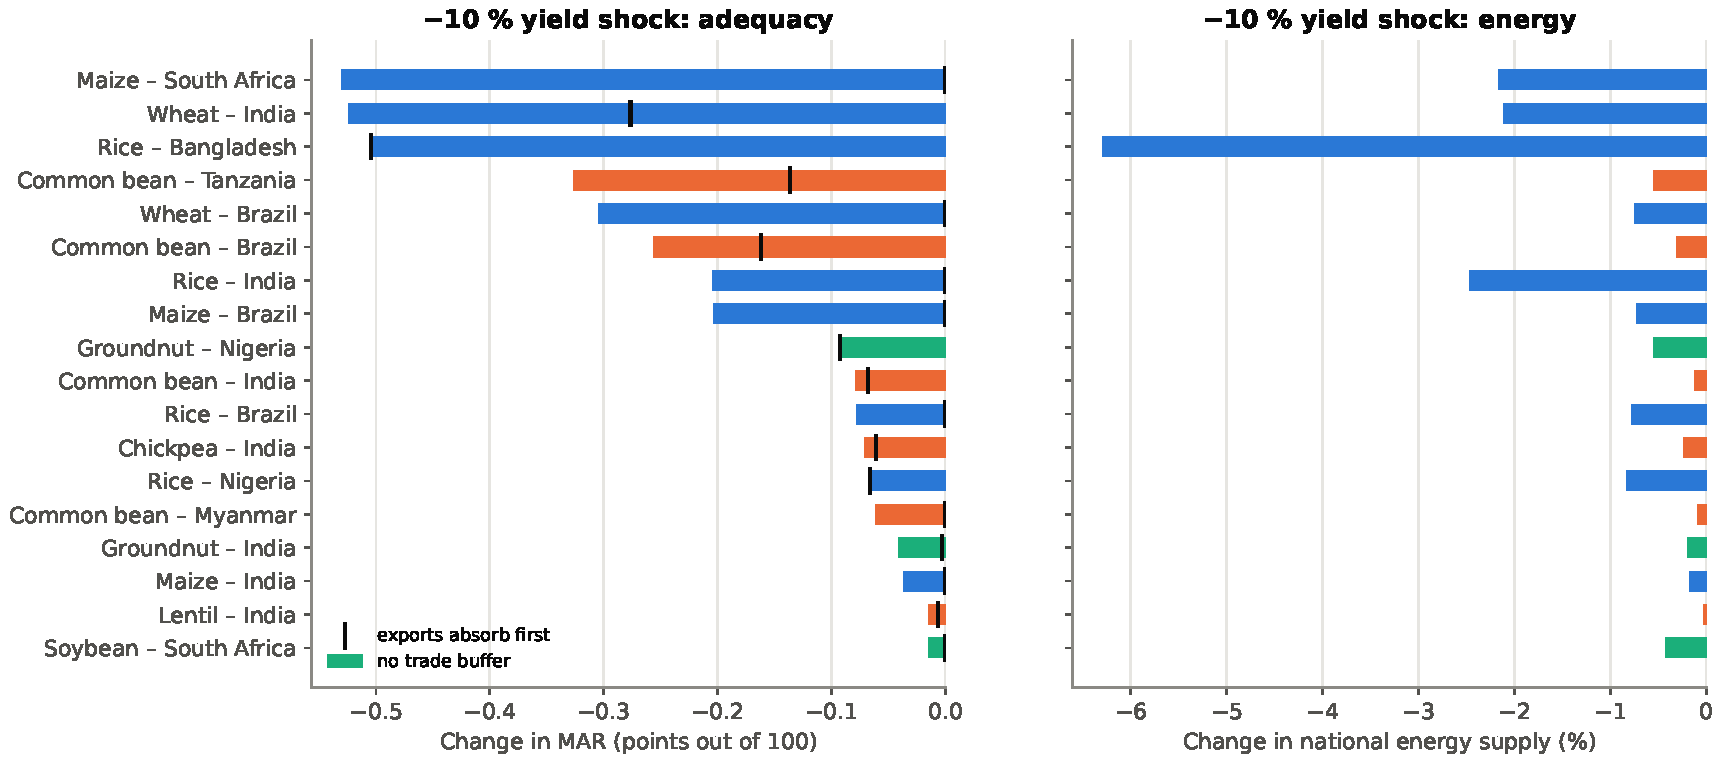
\includegraphics[width=0.95\linewidth]{G08_yield_shock.pdf}
\caption{Standard $-10\%$ yield loss: change in national energy supply and in MAR for the pairs with the largest
MAR change (upper bound and export-buffered lower bound).}\label{fig:shock}\end{figure}

\paragraph{MAR.} Removing 10\% of a crop's production share of supply changes national MAR by less than 0.005
points in \shockZeroMar\ of \shockN\ pairs. This is because national supply stays above requirement for most
nutrients.
\begin{itemize}
\item The largest MAR fall is \shockTopMar\ (\shockTopMarValue\ points).
\item The largest energy loss is \shockTopKcal\ (\shockTopKcalValue\% of national kcal).
\end{itemize}
Because MAR caps each ratio at one, it hides losses that still leave supply above requirement, so the nutrient
losses themselves are reported alongside (Figure~\ref{fig:shock}, Table~\ref{tab:shock}). The largest MAR changes
come where iron is already short and the shocked crop is an iron source.

\paragraph{History.} In the old food balance sheets (1961--2013), a bad harvest significantly lowered food supply
in \passOldPos\ of \passOldN\ pairs; in the new series (2010--2023), in \passNewPos\ of \passNewN.
\begin{itemize}
\item These are associations. Trade and stocks buffer most losses.
\item The new series has only 14 years, so an insignificant estimate there is not proof of buffering.
\end{itemize}

\subsection{Conditional future yield and nutrient change}\label{sec:futurenut}
\begin{figure}[H]\centering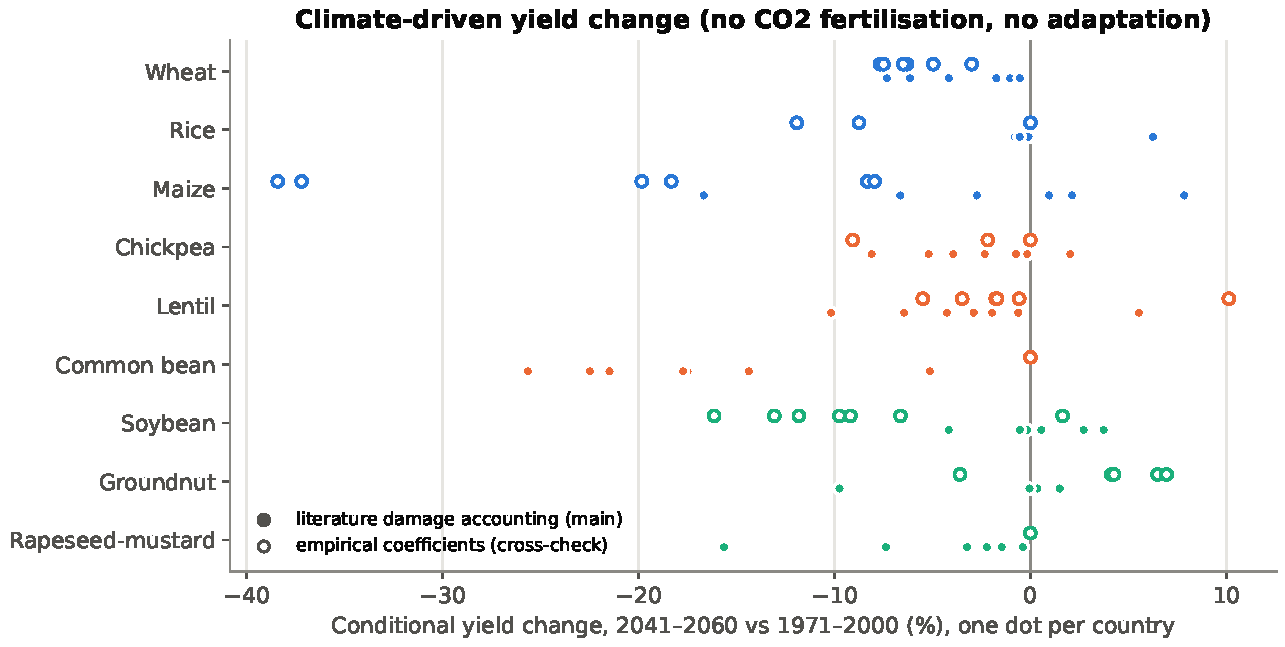
\includegraphics[width=0.9\linewidth]{G09_future_yield.pdf}
\caption{Climate-driven yield change 1971--2000 $\to$ 2041--2060 by crop: literature damage accounting (main)
and empirical coefficients (cross-check).}\label{fig:futyield}\end{figure}

\paragraph{Main estimate.} The literature damage accounting (Section~\ref{sec:futureyield}) gives a yield loss in
\fyLitNeg\ of \fyN\ pairs.
\begin{itemize}
\item The largest mean loss by crop is for \futYieldWorst\ (\futYieldWorstValue\%), driven by heat during
flowering.
\item The largest nutrient consequence is \futNutTopPair\ (MAR \futNutTopMar\ points)
(Table~\ref{tab:futyield}, Table~\ref{tab:futnut}).
\end{itemize}

\paragraph{Empirical cross-check.} The empirical coefficients give a loss in \fyEmpNeg\ of \fyN\ pairs and
detect any climate response in \fyEmpDetected\ of \fyN.
\begin{itemize}
\item The two methods agree in sign for \fySameSign\% of pairs.
\item Their pair-level rank correlation is \corrLitEmp.
\end{itemize}

\paragraph{Why they differ.}
\begin{itemize}
\item The literature functions describe yield damage above a threshold under controlled conditions.
\item The regressions describe how national yields co-varied with monthly climate in 1971--2000, including
adaptation and irrigation, with few statistically clear heat effects.
\item Common bean has the largest literature loss but no detectable empirical climate response in any of its
countries.
\item Maize shows the opposite contrast. Its empirical coefficients imply much larger losses than the literature
accounting. Its fitted heat coefficients are steep (the US and South African country estimates and the pooled
panel estimate used elsewhere), while maize's literature threshold of \SI{32}{\celsius} on monthly $\Teff$ is
rarely crossed.
\end{itemize}
Neither method is validated against future yields. Their disagreement is the main uncertainty in the future
nutrient numbers.

\paragraph{Status.} The future nutrient numbers are therefore reported as a \textbf{conditional screening
estimate}: what the literature damage functions imply under one climate model with today's crop area and diets.
They are not a forecast, and they are not confirmed by the observed yield record.

\begin{table}[H]\centering\small\caption{Conditional climate-driven yield change by crop, 1971--2000 $\to$
2041--2060 (literature accounting and empirical cross-check).}\label{tab:futyield}
\adjustbox{max width=\linewidth}{\begin{tabular}{lrrrr}
\toprule
Crop & $\Delta T_{eff}$ \si{\celsius} & $\Delta Y$ lit (mean \%) & range over countries & $\Delta Y$ empirical (mean \%) \\
\midrule
Wheat & +2.0 & -3.5 & -7.3 to -0.5 & -6.0 \\
Rice & +1.8 & +0.7 & -0.8 to +6.3 & -3.0 \\
Maize & +2.0 & -2.5 & -16.7 to +7.8 & -21.7 \\
Chickpea & +2.0 & -2.6 & -8.1 to +2.0 & -1.6 \\
Lentil & +2.2 & -3.0 & -10.2 to +5.5 & -0.7 \\
Common bean & +2.0 & -17.8 & -25.6 to -5.1 & +0.0 \\
Soybean & +1.9 & +0.7 & -4.2 to +3.7 & -9.3 \\
Groundnut & +1.6 & -1.3 & -9.7 to +1.5 & +3.6 \\
Rapeseed-mustard & +2.0 & -5.4 & -15.6 to -0.4 & +0.0 \\
\bottomrule
\end{tabular}
}\end{table}
